% !TeX root = main.tex

\subsection{Homology} % (fold)
\label{sec:homology}

Simplicial complexes not only provide a comprehensive discretization of continuous domains, but are the primary tool for concrete calculations in algebratic topology.
In particular, the study of simplicial homology groups rely on simplicial complexes in order to study important topological invariants of a discretized space.

The following vector spaces may be defined over any field $\F$, however we will assume the field $\F_2$ in order to avoid orienting the simplices in $K$.
Let $C_k(K)$ denote the vector space over some field $\F$ consisting of linear combinations of $k$-simplices in $K$, which form a basis for $C_k(K)$, known as \textbf{$k$-chains}.
These vector spaces are connected by \textbf{boundary maps} $\partial_k:C_k(K)\to C_{k-1}(K)$ which are linear transformations taking basis elements of $C_k(K)$ to the abstract sum of basis $(k-1)$-simplex faces.
The collection of chains and boundary maps forms a sequence of vector spaces known as the \textbf{chain complex} $\C = (C_*,\partial_*)$
\[
    \ldots\xrightarrow{\partial_{k+1}}
    C_k(K)\xrightarrow{\partial_{k}}
    C_{k-1}(K)\xrightarrow{\partial_{k-1}}
    \ldots\xrightarrow{\partial_2}
    C_1(K)\xrightarrow{\partial_{1}}
    C_0(K)\xrightarrow{\partial_0} 0.
\]

An important property of the boundary maps $\partial_k$ is that the composition of subsequent boundary maps is zero.
That is, for all $k$
\[
  \partial_k\circ\partial_{k-1} = 0.
\]
As a result the image of $\partial_{k+1}$, denoted $\im\partial_{k+1} = \{\partial_{k+1}c\mid c\in C_{k+1}(K)$ is a subspace of the kernel, $\ker\partial_k = \{c\in C_k(K)\mid \partial_k c = 0\}$, of $\partial_k$.
A \textbf{$k$-cycle} of $\C$ is a $k$-chain with empty boundary---an element of $\ker\partial_k$.
Two cycles in $\ker\partial_k$ are said to be \textbf{homologous} if they differ by an element of $\im\partial_{k+1}$.
This leads us to the definition of the homology groups of $K$ as quotient vector spaces $H_k(K)$ over $\F$.

\begin{definition}
    For $k\in\N$ the \textbf{$k$th homology group} of a simplicial complex $K$ is the quotient group
    \[ \hom_k(K) = \ker\partial_k/\im~\partial_{k+1}. \]
\end{definition}

The rank of a homology group is of particular importance and is known as the \textbf{Betti number} $\beta_k = \rank~ \hom_k(K)$.
These topological invariants can be thought of as counting the number of $k$-dimensional ``holes'' in a topological space, where $0$-dimensional holes are connected components, $1$-dimensional holes are loops, $2$-dimensional holes are voids, and so on.
Note that this is the same notion which motivated our use of simplicial complexes for determining coverage---a $1$-dimensional hole exists if a gap in a neighborhood graph cannot be filled by triangles.

\paragraph*{\textbf{Relative Homology}}

\figblock{%
\begin{figure}[htbp]
\centering
    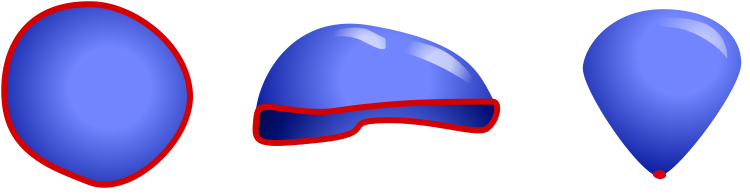
\includegraphics[scale=0.5]{figures/balloons1.png}\vspace{2ex}
    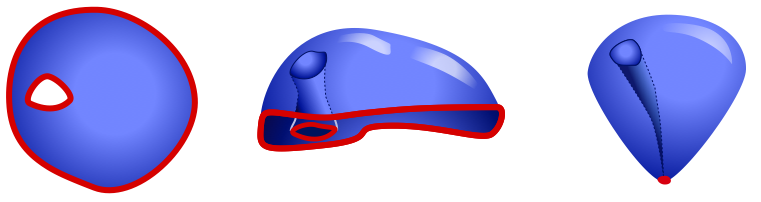
\includegraphics[scale=0.5]{figures/balloons3.png}
    \caption{(Left) Two connected, planar domains with boundaries (in red).
            We can gather some intuition for the relative homology of a pair $(\D,\B)$ by thinking about wrapping the interior of the domain around its boundary, and identifying all points in the boundary with a point (Right).
            Even with disconnected boundaries we know that $\beta_2 = \rank~ H_2(\D, \B) = 1$.  That is, there is just one enclosed void.}
    \label{fig:balloons1}
\end{figure}}

For a simplicial complex $K$ let $L\subset K$ be a subcomplex of $K$.
Let $\C(K, L)$ denote the quotient chain complex of pairs $(C_k(K, L), \overline{\partial_k})$ where $C_k(K, L) = C_k(K)/C_k(L)$ consists of the chains on $K$ modulo chains on $L$, with the induced boundary maps $\overline{\partial_k}$ on the quotients.
Each relative chain is an equivalence class of chains in $K$ which are identical without the elements of $L$.
The \textbf{relative homology groups} $\hom_k(K, L)$ consist of homology classes of relative cycles---chains in $K$ whose boundaries vanish or lie in $L$.
That is, a relative cycle can either be a cycle in $K$ or a chain in $K$ with a boundary in $L$.

\begin{theorem}[Excision]\label{thm:excision}
    Let $X$ be a topological space and $A$ and $U$ be subspaces such that $U$ is also a subspace of $A$.
    If $\cl(U)\subseteq \intr(A)$ then $\hom_*(X\setminus U, A\setminus U)\cong \hom_*(X, A)$.
\end{theorem}

\begin{corollary}
    If $\intr(A)\cup \intr(B) = X$ then $\hom_*(X, A)\cong \hom_*(B, A\cap B)$.
\end{corollary}

% section homology (end)
